% Preprint version 2 (revised after reader feedback, Sept 2026).
% Build: tectonic preprint_v2.tex
\documentclass[12pt,letterpaper]{article}
\usepackage[T1]{fontenc}
\usepackage[utf8]{inputenc}
\usepackage{newtxtext,newtxmath}
\usepackage[margin=1in]{geometry}
\usepackage{setspace}
\usepackage{graphicx}
\usepackage{float}
\usepackage{caption}
\usepackage{booktabs}
\usepackage{array}
\usepackage{pgfplots}
\usepackage[hidelinks]{hyperref}
\usepackage{url}
\pgfplotsset{compat=1.18}
\usetikzlibrary{positioning,arrows.meta,calc}
\graphicspath{{../../figures/}{../../data/interim/comparison_sheets/}}
\captionsetup[table]{name=Table,labelsep=period,justification=raggedright,singlelinecheck=false,skip=4pt}
\captionsetup[figure]{name=Fig.,labelsep=period,justification=raggedright,singlelinecheck=false,skip=6pt}
\setlength{\parindent}{0.5in}
\emergencystretch=1.5em
\title{Three Ways to Miss a Grasp}
\begin{document}
\setstretch{1.1}

% ---------------- Title, author, abstract, keywords ----------------
\begin{center}
{\Large\bfseries Three Ways to Miss a Grasp: A Same-Metric Comparison of
Rule-Based, Learned, and Zero-Shot Vision-Language Grasp Prediction, and a
Test of Why the Language Model Fails\par}
\vspace{0.2in}
{\large Anish Talla\par}
{Lightridge High School and Academies of Loudoun, Virginia, United States\par}
{\texttt{anish.talla99@gmail.com}\par}
\vspace{0.1in}{\small Preprint, version 2, September 2026. Code and data: \url{https://github.com/anishtalla27/Vision-Based-Grasping}\par}
\end{center}
\vspace{0.2in}
\section*{Abstract}\addcontentsline{toc}{section}{Abstract}

A robot cannot grasp an object until something decides where to place
the fingers and at what angle. That decision can come from hand-written
rules, from a network trained on labeled grasps, or from a
general-purpose vision-language model never trained on grasping, and the
three are rarely compared under one protocol. This paper scores one
system of each kind with a single implementation of the Cornell
rectangle metric on the same held-out split of 123 images of 35 unseen
objects, with object-clustered statistics and a shared failure taxonomy.
A fine-tuned ResNet34 passed on 84.0\% of test images (three-seed mean),
a detector-plus-lookup-table heuristic on a post-hoc-corrected 57.7\%,
and zero-shot GPT-4o on 12.4\%. The systems also failed in different
ways, and GPT-4o's errors suggested that it could identify a grasp but
not express it as pixel coordinates. A follow-up experiment tested that
account by asking the same model to choose among label-free candidate
grasps drawn on the image. Its accuracy stayed at the random floor on
three candidate menus, and it consistently preferred a pinch along the
object's long axis. Removing the coordinate output does not recover
performance, which points to the grasp choice itself, although
difficulty interpreting the drawn marks cannot yet be excluded.


\section*{Keywords}\addcontentsline{toc}{section}{Keywords}
robotic grasping; Cornell Grasping Dataset; convolutional neural networks;
vision-language models; GPT-4o; Set-of-Mark prompting; zero-shot evaluation;
object-clustered bootstrap; failure analysis; spatial grounding

\section{Introduction}

Before a gripper closes on anything, something has to choose a contact
point, an approach angle, and how wide to open the fingers. Every
subsequent motion depends on that choice being approximately correct. A
mechanically capable arm will still fail often if the component that
selects the grasp is wrong, so grasp prediction is a stage at which a
small difference in accuracy produces a large difference in behavior.
The decision must also be made from limited information. In most
practical settings the robot has a camera image but no model of the
object and no label identifying it.

Three broadly different approaches exist, and they are not variations on
a single method. A programmer can encode rules directly, for example
that a mug is grasped by its handle and a bottle around its neck. A
model can be trained on thousands of hand-labeled examples until it
learns to map pixels to grasp rectangles. Alternatively, a
general-purpose vision-language model, trained on web text and images
and never shown a grasping dataset, can be asked in natural language
where to grip. Each approach places the relevant knowledge in a
different part of the perception stack, whether explicit rules, weights
fitted to task-specific data, or the general knowledge of a large model.

The third option is recent, and the field has not settled how to use it.
Foundation models entered robotics quickly, and the literature has not
yet established which parts of a manipulation pipeline they should
handle. The question matters practically, because the three approaches
demand very different resources. A lookup table needs only
hand-specified rules, and a learned predictor needs a task-specific
annotated dataset and the compute to train on it, whereas prompting a
hosted vision-language model requires only an API key and minimal setup.
Because that convenience makes the approach attractive, its accuracy
should be measured before it is relied on.

Comparisons across those three families are rare. Most published
grasp-detection work benchmarks within a family, comparing one trained
architecture against another on the same dataset. Such benchmarks are
useful, but they do not show what is gained or lost by changing approach
entirely. Rule-based baselines, when they appear, are often described
but not scored. Vision-language models usually appear embedded inside a
larger system, where their individual contribution cannot be isolated.
This study evaluates all three on the same test images, with a common
output format and a single scoring implementation.

This paper asks which approach works and where each one breaks down. The
second question is treated as equal to the first, because an accuracy
figure shows only that a system was wrong, while the pattern of its
errors points to a cause that a designer can act on.

The evaluation protocol is adopted from prior work. A grasp here is a
rectangle with a center point, an orientation, and a width matched to
how far the gripper opens, the representation Jiang et
al.~\cite{jiang2011} introduced with the Cornell Grasping Dataset. Each
image has several labeled grasps, since most objects can be picked up in
more than one valid way, and a prediction counts as correct if it
matches any of them. The matching rule is that the predicted angle falls
within 30 degrees of a labeled grasp and the intersection over union
between the two rectangles exceeds 25\%, the convention established by
Lenz et al.~\cite{lenz2015}. An external ground truth was used because
an earlier design, in which the author would have written the ground
truth and then graded a rule-based system against it, was close to
circular. The dataset's existing annotations avoid that problem and make
the results comparable to published ones.

Four systems are evaluated. System A is the rule-based baseline, in
which a COCO-pretrained detector identifies the object and a small fixed
table maps the detected category to a grasp region, with a geometric
fallback covering the images the detector cannot name. System B is the
learned predictor, a small convolutional network built from scratch
alongside fine-tuned ResNet18 and ResNet34 models, trained on the
Cornell training split. System C is GPT-4o, prompted directly with the
raw image and given no task-specific training. System D is the same
model shown a menu of candidate grasps drawn on the image and asked only
to choose one, a follow-up run added after the first three systems were
scored, to test the explanation their results suggested.

This paper does not attempt to improve on state-of-the-art grasp
detection, and published pixel-wise systems reach higher accuracies than
any system evaluated here. Its aim is to measure, under conditions held
as close to identical as the design allows, how three families of
technique fail, and to show that the pattern of each failure contains
information that the accuracy figure does not.

This paper makes the following contributions.
\begin{enumerate}
\item A same-metric comparison of a rule-based, a learned, and a
zero-shot vision-language grasp predictor, run on the same 123 held-out
images of unseen objects through one shared scoring path.
\item Uncertainty reported at the level of the object, the unit that matches the stated population of unseen objects. The ordering of the three systems is preserved under an object-clustered bootstrap and permutation test, and the learned system is reported over
three seeds under selection rules fixed before the test split was
reopened.
\item A failure taxonomy and a center-hull diagnostic that separate the
three families along lines a single accuracy number does not show.
\item A marked-candidate experiment (System D) with a floor and a
ceiling computed on its own menu. It tests the most natural explanation of the vision-language model's
failure, that the model cannot express a chosen grasp as coordinates,
and shows that removing the coordinate output is not sufficient to
recover performance.
\item A public release of the code, the object-wise split, and every
raw model reply.
\end{enumerate}

% ===============================================================

\subsection{Relation to prior work}

This study builds on existing components: the Cornell Grasping Dataset
and its rectangle representation~\cite{jiang2011}, the 30-degree and
25\% IoU pass rule~\cite{lenz2015}, the ResNet architectures with
ImageNet weights~\cite{he2016}, Faster R-CNN with COCO
weights~\cite{ren2015}, the sine and cosine encoding of twice the grasp
angle~\cite{redmon2015,morrison2018}, GPT-4o~\cite{openai2024}, and
marked-candidate prompting~\cite{yang2024}. The work specific to this
study is the shared evaluation pipeline, the reconstruction of object
identities and the object-wise split, the detector-plus-table baseline,
the training recipe and pre-registered second round of the learned
system, the five-repeat protocol for the zero-shot model, the failure
diagnostics, the object-clustered statistical analysis, and the
candidate generator and menus that make up System D.

\section{Methods}\label{sec:methods}

Fig.~\ref{fig:overview} summarizes the design. Every system receives the
same RGB test image and must return the same kind of output, a grasp
rectangle, which is scored by one function against the dataset's labeled
grasps. This section describes the design only. All numbers are reported
in Section~\ref{sec:results} and interpreted in
Section~\ref{sec:discussion}.

\begin{figure}[H]
\centering
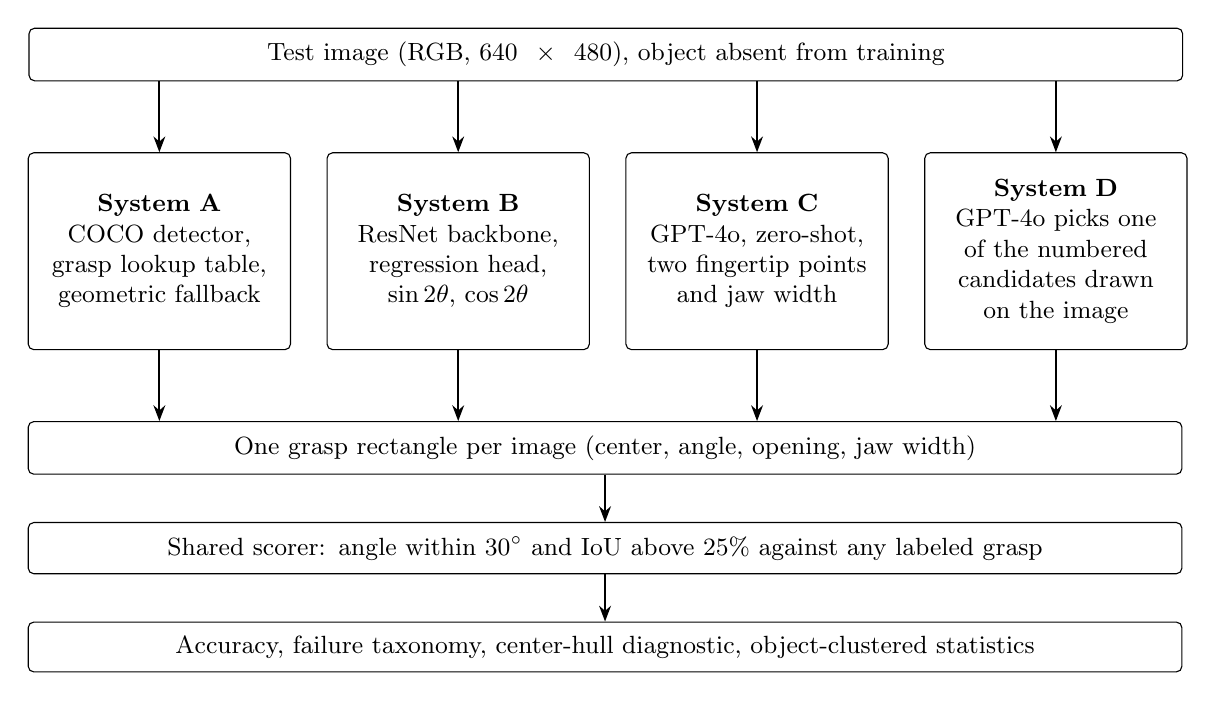
\begin{tikzpicture}[
  font=\small,
  box/.style={draw, rounded corners=2pt, align=center, inner sep=4pt,
              text width=3.05cm, minimum height=2.5cm},
  wide/.style={draw, rounded corners=2pt, align=center, inner sep=5pt,
               text width=14.3cm},
  arr/.style={-{Stealth[length=2mm]}, thick},
]
\node[wide] (img) {Test image (RGB, $640\times480$), object absent from training};
\node[box, below=0.9cm of img, xshift=-5.67cm] (A)
  {\textbf{System A}\\COCO detector, grasp lookup table, geometric fallback};
\node[box, right=0.45cm of A] (B)
  {\textbf{System B}\\ResNet backbone, regression head, $\sin2\theta$, $\cos2\theta$};
\node[box, right=0.45cm of B] (C)
  {\textbf{System C}\\GPT-4o, zero-shot, two fingertip points and jaw width};
\node[box, right=0.45cm of C] (D)
  {\textbf{System D}\\GPT-4o picks one of the numbered candidates drawn on the image};
\node[wide, below=0.9cm of A.south west, anchor=north west] (rect)
  {One grasp rectangle per image (center, angle, opening, jaw width)};
\node[wide, below=0.6cm of rect] (score)
  {Shared scorer: angle within $30^\circ$ and IoU above 25\% against any labeled grasp};
\node[wide, below=0.6cm of score] (out)
  {Accuracy, failure taxonomy, center-hull diagnostic, object-clustered statistics};
\foreach \s in {A,B,C,D} {
  \draw[arr] (img.south -| \s.north) -- (\s.north);
  \draw[arr] (\s.south) -- (\s.south |- rect.north);
}
\draw[arr] (rect) -- (score);
\draw[arr] (score) -- (out);
\end{tikzpicture}
\caption{Overview of the comparison. The four systems differ only in how
the grasp rectangle is produced. Everything below the system row is
shared.}
\label{fig:overview}
\end{figure}

\subsection{Dataset and evaluation}

The dataset used for evaluation is the Cornell Grasping Dataset, roughly
a thousand images of household objects, each with hand-labeled grasp
rectangles~\cite{jiang2011}. A prediction counts as correct when its
angle falls within 30 degrees of some labeled grasp and its rectangle
intersection over union with that grasp exceeds 25\%, the convention
established by Lenz et al.~\cite{lenz2015}. Cornell's annotations are
not exhaustive, so passing this metric shows agreement with a labeled
grasp and does not establish that the grasp would physically succeed.
The Jacquard dataset was considered as an alternative, but its full
distribution requires a signed agreement and an approved non-free-email
request. Reconstructing object identity was the most difficult step in
building the split. No object may appear in both training and test, or a
model can memorize its grasp rectangles from one split and be credited
for recognizing the same object in the other. Cornell provides no
object-identity labels, so identity had to be reconstructed from the
image sequence. Comparing raw pixel differences between consecutive
frames failed, because the dataset deliberately rotates each object
between shots and same-object and different-object scores overlapped.
Instead, each frame was segmented against the photography platform, and
the resulting object regions were compared to decide whether two frames
showed the same object or different ones.

Acceptance thresholds were set asymmetrically, since merging two
different objects into one group is less harmful than splitting one real
object into two. The ``different-object'' threshold was set below the
lowest score seen for any confirmed same-object pair, while the
``same-object'' threshold was left permissive. A 30-boundary stratified
sample was classified by both an AI assistant and a human, blind to each
other's calls. The AI's classifications matched the human's on 86.7\% of
its confident calls but only 40.0\% of the calls it flagged as
uncertain, so every uncertain call and every confident ``different''
call was reviewed by hand. Confident ``same'' calls were accepted
unreviewed, since an error in that direction is harmless. The result is
234 objects across 883 images, with 620 for training, 140 for
validation, and 123 for test, as shown in Table~\ref{tab:split}.
Published descriptions of Cornell normally report around 240 objects,
and the shortfall here is expected, since the thresholds were
deliberately biased toward merging. Every merge that should have been a
split lowers the object count while keeping the merged group on one side
of the division, which is the direction of error this design
deliberately accepts. Each object has at least one grasp rectangle, and
most have several, since most objects can be picked up more than one
way.

\subsection{System A, rule-based baseline}

System A is better described as a detector-assisted heuristic baseline
than a purely rule-based one. It detects the object with a
COCO-pretrained detector, which is itself a learned component, then
looks up the detected category in a fixed table of grasps. No part of it
is learned from grasp labels, which is the sense in which it is
rule-based. The table was committed before any evaluation code existed,
so no entry could be tuned toward a score. Since COCO's categories miss
more than half of what Cornell photographs, a geometric fallback that
does not rely on object recognition covers the objects the detector
misses, and that fallback handles the majority of test images.

System A was scored once before the detector was found to be drawing
boxes around background clutter. The guard that corrected this, a
requirement that the detected box contain the object's centroid together
with one constant recalibrated on training data, was added after those
test predictions had been inspected. The decision to add it was
therefore prompted by test behavior, and the corrected figure is a
post-hoc result. This weakens the comparisons that rest on it, including
the McNemar test against System B and the interval comparison against
System C. Both the original and the corrected figure are reported
wherever the result appears (Section~\ref{sec:res-a}).

COCO's 80 categories do not cover most of the objects in Cornell, so
many objects have no table entry. In addition, on either path System A's
rectangle orientation is limited to 0 or 90 degrees, the only two
orientations the table and the box-based rule can express, so it cannot
produce a grasp that requires an intermediate angle.

\subsection{System B, learned grasp predictor}

System B regresses a grasp rectangle directly from an image. A backbone
network extracts features, pools them, and a regression head predicts
the rectangle's parameters. Orientation is encoded as the sine and
cosine of twice the angle rather than a raw angle between 0 and 180
degrees. This accounts for the fact that a grasp rectangle rotated 180
degrees describes the same physical grasp. A raw-angle representation
would score that rotation as an entirely different grasp, while the sine
and cosine encoding treats it as identical. Redmon and
Angelova~\cite{redmon2015} and Morrison et al.~\cite{morrison2018} both
used this same encoding.

System B trained three architectures on the same training split, a small
network built from scratch, a fine-tuned ResNet18, and a fine-tuned
ResNet34. The loss was computed against every labeled grasp on an image,
with only the best match backpropagated. Averaging over all of an
image's grasps would place the target between, for example, a handle
grasp and a rim grasp, at a point where neither is valid. Augmentation
applied the same affine transform to the grasp rectangle's corners as to
the image's pixels, instead of hand-writing a rule for how the angle
behaves under a flip.

System B was trained twice. The first round trained each architecture
once, at one seed, with a constant learning rate, and kept whichever of
roughly a hundred epochs scored highest on validation. Validation
accuracy on 140 images varies substantially between consecutive epochs
(Section~\ref{sec:res-b}), so the maximum over epochs is a noisy
selection criterion and a single run cannot separate one architecture
from another. The second round kept the model, loss, data, metric, and
split, and changed only the recipe: a cosine learning-rate decay over a
fixed 100 epochs, an exponential moving average of the weights, three
seeds per architecture, and no checkpoint selection at all, since the
reported model is the final-epoch averaged weights. Test-time
augmentation, eight dihedral views of each image with the prediction
carried back through the same corner transform used in training and the
medoid rectangle kept, was added and its use decided on validation. Four
rules were fixed before the second round was evaluated on the test
split: the architecture is the one with the higher mean final-weight
validation accuracy across seeds, augmentation is used only if it raises
that mean, the primary result is the mean over seeds of the final
weights, and every configuration evaluated on the test split is
reported. A 60-epoch budget was tried first and rejected on validation
alone, since both architectures were still improving when the decay
ended. Opening the test split a second time departs from the original
single-opening plan.

\subsection{System C, zero-shot vision-language model}

System C prompts GPT-4o with each test image and asks where the two
gripper fingertips should touch, with no training or fine-tuning on
grasping. The prompt was developed on a batch of 30 training images and
frozen before test was opened.

The model was called as
\texttt{openai/gpt-4o} through the OpenRouter API, at a 400-token cap,
with temperature left unset so the provider default applied and no seed
pinned, since run-to-run variation was one of the quantities being measured. Images were sent at the dataset's native 640 by 480
resolution with no resizing, and the prompt told the model that
coordinates were in pixels of that image. Each repeat was an
independent single-turn completion with no prior messages, so the five repeats of an image are independent draws. Transport failures were retried up to three times, but a
reply that arrived and then failed to parse was never retried, since resampling malformed replies would implicitly convert a
single-shot baseline into a best-of-N one.

System C was not asked to output an angle. It returned two fingertip
points and a jaw width as JSON, and those three values determine all
four rectangle corners, which were then passed through the same frozen
function that produced every ground-truth angle in the dataset. No
rectangle parameter was supplied manually, and no angle convention had
to be matched. Each image was prompted five times, and all five results
are reported.

The design isolates one step that published systems usually avoid. In
several grasping systems built on the same kind of model, the model's
output is a choice, a label, an order of operations, or an image, and
the pose of the gripper comes from something else. FreeGrasp asks the
model to decide which object to grasp and in what order, using marks
placed on the image~\cite{jiao2025}. Lan-grasp asks the model which part
to grasp, then hands the pose to a conventional
planner~\cite{mirjalili2023}. ThinkGrasp uses the model to plan clutter
removal~\cite{qian2024}. Set-of-Mark asks the model to select one of
several labeled regions~\cite{yang2024}. VLAD-Grasp asks the model to
draw the grasp using a virtual gripper~\cite{kulshrestha2025}. In none
of them does the model emit the pose coordinates itself. System C asks
for exactly that, so that any gap can then be examined as a failure of
coordinate emission or as a failure to perceive the object.

\subsection{System D, marked-candidate selection}

System D tests the coordinate-binding account directly. If GPT-4o can
see where to grasp but cannot express it as pixel coordinates, then
removing the coordinate output should recover its choice. The same model
was therefore shown the same test images with twelve candidate grasps
drawn on a zoomed crop of the object and asked to return the number of
the one it would use. In this setting the model never emits a
coordinate.

The candidates are generated without reading any grasp label. The
platform segmentation already used for the object-wise split gives the
object's mask, and principal component analysis of that mask gives its
centroid, long axis, and extent. Candidates are three positions along
the long axis (the centroid and 35\% of the extent to either side)
crossed with four jaw-travel directions 45 degrees apart, starting from
the short axis, so every possible grasp angle lies within 22.5 degrees
of some candidate, inside the metric's 30 degree tolerance. Opening and
jaw width use System A's train-calibrated constants. Each candidate is
drawn as two thick fingertip pads joined by a thin line with inward
arrowheads, in its own color, with a numbered badge. The numbering is
re-shuffled on every call, so a preference for a particular number
cannot be mistaken for a preference for a grasp, and self-agreement is
measured on the physical candidate. Eleven test images have no
segmentation mask and so no candidates. They count as misses for System
D and for every reference row it is compared with, so the comparisons
stay paired.

\begin{figure}[H]
\centering
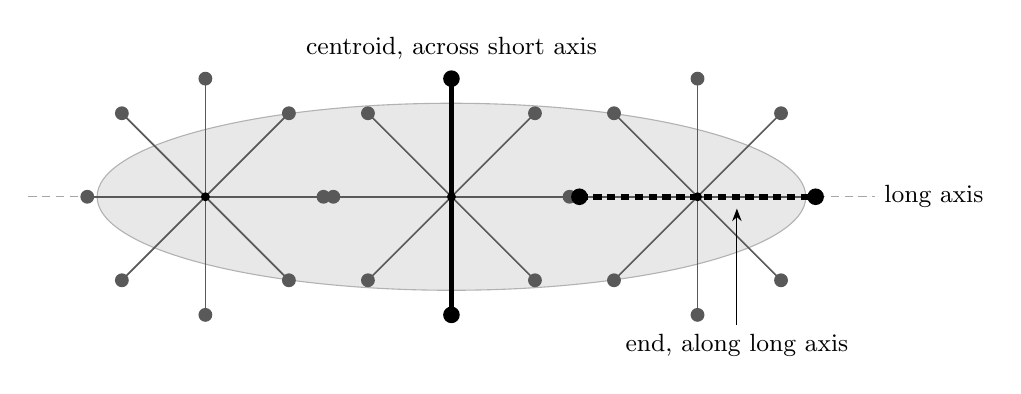
\begin{tikzpicture}[font=\small, scale=1.25]
\fill[gray!18] (0,0) ellipse (3.6 and 0.95);
\draw[gray!60] (0,0) ellipse (3.6 and 0.95);
\draw[densely dashed, gray!70] (-4.3,0) -- (4.3,0) node[right, black] {long axis};
\foreach \x in {-2.5,0,2.5} {
  \foreach \a in {90,45,0,135} {
    \draw[black!65, semithick] ($(\x,0)+(\a:1.2)$) -- ($(\x,0)+(\a+180:1.2)$);
    \fill[black!65] ($(\x,0)+(\a:1.2)$) circle (2pt);
    \fill[black!65] ($(\x,0)+(\a+180:1.2)$) circle (2pt);
  }
  \fill[black] (\x,0) circle (1.3pt);
}
% centroid, short axis
\draw[line width=2pt] (0,1.2) -- (0,-1.2);
\fill (0,1.2) circle (2.4pt); \fill (0,-1.2) circle (2.4pt);
\node[above] at (0,1.3) {centroid, across short axis};
% end, long axis
\draw[line width=2pt, densely dashed] (1.3,0) -- (3.7,0);
\fill (1.3,0) circle (2.4pt); \fill (3.7,0) circle (2.4pt);
\node[below] at (2.9,-1.3) {end, along long axis};
\draw[-{Stealth[length=1.6mm]}] (2.9,-1.3) -- (2.9,-0.12);
\end{tikzpicture}
\caption{Schematic of the twelve-candidate menu, not to scale. The
object mask (gray) gives a centroid and a long axis. Candidates are
three positions along that axis crossed with four jaw-travel
directions, and each line joins the two fingertip pads of one
candidate. The solid candidate is the label-free geometric rule. The
dashed candidate is the end pinch discussed in
Section~\ref{sec:discussion}. The model sees the candidates drawn in
color on the photograph with shuffled numbers, as in
Fig.~\ref{fig:som}.}
\label{fig:menu}
\end{figure}

Because the menu is fixed before the model sees it, the run comes with
its own floor and ceiling computed on the same candidates: the expected
accuracy of a uniformly random choice, and whether any candidate passes
at all. It also yields, as a by-product, a fourth non-learned baseline,
the candidate at the centroid closing across the short axis, which
unlike System A can express a diagonal grasp.

The prompt was developed on the same 30 training images System C used,
two repeats each, and judged on parse rate and on whether the model was
reading the glyph as intended. The first version drew each candidate as
a thin line with small end ticks. The model frequently chose the
candidate running along the object's long axis while describing a grasp
``across the narrowest part'', which could have meant it was reading the
line as the finger plates instead of the closing direction. The second
version drew explicit pads and arrowheads and described them in the
prompt. The behavior did not change (Section~\ref{sec:res-d}), which
suggests that the test result reflects the model's preference and is
unlikely to be an artifact of that particular glyph. Accuracy on the
development images was not used to choose between the versions. The
second version was frozen, and the test split was called once, five
times per image.

After that run, mark size remained as a possible confound. On thin
objects the correct marks are drawn with the small opening the labels
themselves use, so they are the smallest marks on the image, and a
preference for large marks would mimic a preference for the long-axis
grasp. Two further runs address it. Both use four candidates at the
centroid only, the short-axis direction and three rotations of it, so
position is removed and the end-straddling candidates do not exist. In
the first, each mark is drawn at its real opening. In the second, the
same four candidates with the same scored geometry are drawn at one
uniform length, and the prompt gains a single sentence saying the length
is not to scale. Each was parse-checked once on the 30 training images
and then called on the test split five times per image, under its own
sentinel.

\subsection{Stratified analyses}

Each system's design predicts something different about how orientation
should affect it. System A's representation cannot express a diagonal
grasp, System B's encoding handles rotation by construction, and System
C's design makes no prediction in either direction.

An image counts as axis-aligned when any one of its labeled grasps sits
within 15 degrees of 0 or 90 degrees, and as diagonal only when none
does. The rule is deliberately conservative, since a system that can
emit only axis-aligned rectangles still has a valid target whenever a
single labeled grasp is axis-aligned. It is also looser than the 30
degree scoring tolerance, so a diagonal image whose labeled grasps sit
20 degrees off axis is still reachable by an axis-aligned prediction.
Only System A's direction on this split was predicted before the stratum
was scored.

A second split, by the number of grasps labeled per image, was examined
as a difficulty proxy, on the expectation that more labeled grasps give
a prediction more chances to match.

\subsection{Diagnostics and statistical analysis}

Two diagnostics are computed for every system from the output of the
shared scorer. The failure taxonomy records whether a missed prediction
failed the angle criterion, the overlap criterion, or both, or whether
no prediction was produced. The center-hull check asks whether each
predicted center fell inside the convex hull of an image's labeled grasp
rectangles, the loosest spatial test a prediction can fail.

Per-system accuracies are reported with 95\% Wilson intervals, and the
paired comparison between Systems A and B uses McNemar's exact test.
System C is tested separately for each of its five runs and the least
significant result is reported. Because the 123 test images are grouped
within 35 objects, these image-level quantities understate the
uncertainty. The primary intervals therefore resample whole objects with
replacement, differences between systems are bootstrapped on the same
resamples, and an object-clustered permutation test accompanies each
difference.

% ===============================================================
\section{Results}\label{sec:results}

\subsection{The data split}

\begin{table}[H]
\centering
\caption{Object-wise split of the Cornell Grasping Dataset. No object
appears in more than one split.}
\label{tab:split}
\begin{tabular}{lrr}
\toprule
Split & Objects & Images \\
\midrule
Train      & 164 & 620 \\
Validation &  35 & 140 \\
Test       &  35 & 123 \\
\midrule
Total      & 234 & 883 \\
\bottomrule
\end{tabular}
\end{table}

The split covers 234 objects across 883 images, divided roughly 70/15/15
by object count. No object appears in more than one split.

Of the 884 frame boundaries examined, 251 (28.4\%) fell into the
ambiguous band. 139 of those were decided by hand, and the remaining 112
were confident same-object calls accepted without review. Six stayed
uncertain after full review. Four carried a lean toward ``same object''
and were resolved that way, and the other two had no lean. One image
from the smaller side of each was dropped instead, accounting for the
883 images retained out of 885.

\subsection{Overall accuracy}

\begin{table}[H]
\centering
\caption{Test accuracy of every system on the same 123 images, with 95\%
object-clustered intervals. Systems C and D are means over five calls
per image.}
\label{tab:summary}
\begin{tabular}{lrr}
\toprule
System & Accuracy & 95\% CI \\
\midrule
A, detector and lookup table (post-hoc corrected) & 57.7\% & [46.2, 68.2] \\
A, before the correction                          & 40.7\% & --- \\
B, ResNet18, round 1, one seed                    & 79.7\% & [70.8, 87.1] \\
B, ResNet34, round 2, three seeds                 & \textbf{84.0\%} & [73.9, 92.1] \\
C, GPT-4o coordinates, one call                   & 12.4\% & [8.0, 17.4] \\
C, best of five calls                             & 35.0\% & [24.6, 45.5] \\
D, GPT-4o choosing among 12 candidates            & 18.7\% & [9.5, 29.7] \\
Label-free short-axis rule                        & 55.3\% & [41.8, 68.0] \\
\bottomrule
\end{tabular}
\end{table}

Table~\ref{tab:summary} collects the main results, and
Fig.~\ref{fig:headline} shows the three main systems.

\begin{figure}[H]
\centering
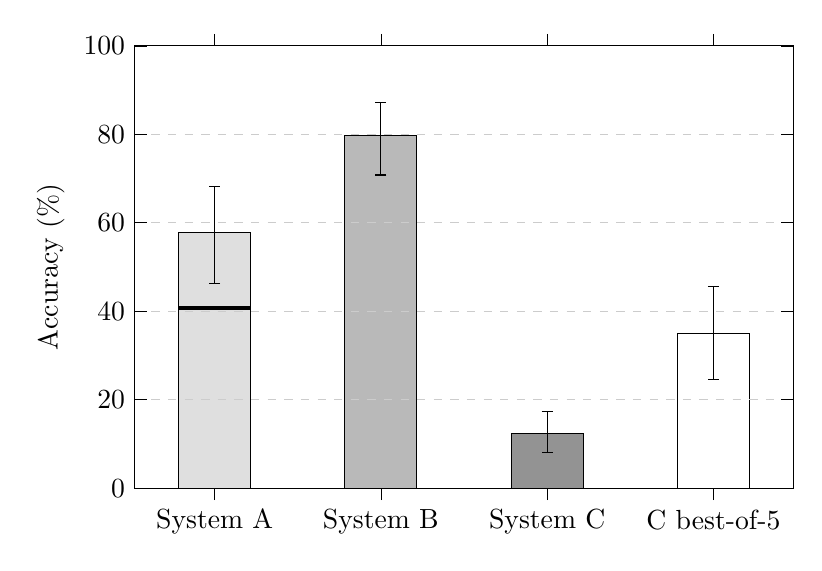
\begin{tikzpicture}
\begin{axis}[
  width=0.82\textwidth, height=7.2cm,
  ybar,
  bar width=26pt,
  ymin=0, ymax=100,
  ylabel={Accuracy (\%)},
  ylabel style={font=\normalsize},
  symbolic x coords={A,B,C,Cb},
  xtick={A,B,C,Cb},
  xticklabels={{System A},{System B},{System C},{C best-of-5}},
  xticklabel style={font=\normalsize},
  yticklabel style={font=\normalsize},
  enlarge x limits=0.16,
  ymajorgrids=true,
  grid style={dashed,gray!40},
  axis on top,
  tick style={black},
]
% each bar placed at its own symbolic x, so shift is suppressed
\addplot[fill=gray!25,draw=black,bar shift=0pt,
  error bars/.cd, y dir=both, y explicit]
  coordinates { (A, 57.7) += (0,10.5) -= (0,11.5) };
\addplot[fill=gray!55,draw=black,bar shift=0pt,
  error bars/.cd, y dir=both, y explicit]
  coordinates { (B, 79.7) += (0,7.4)  -= (0,8.9)  };
\addplot[fill=gray!85,draw=black,bar shift=0pt,
  error bars/.cd, y dir=both, y explicit]
  coordinates { (C, 12.4) += (0,5.0)  -= (0,4.4)  };
\addplot[fill=white,draw=black,bar shift=0pt,
  error bars/.cd, y dir=both, y explicit]
  coordinates { (Cb, 35.0) += (0,10.5) -= (0,10.4) };
% System A before the post-hoc guard was added
\addplot[only marks,mark=-,mark size=13pt,very thick,draw=black]
  coordinates { (A, 40.7) };
\end{axis}
\end{tikzpicture}
\caption{Test-set accuracy with 95\% object-clustered intervals, the
primary intervals in this paper. System A 57.7 [46.2, 68.2], System B
79.7 [70.8, 87.1], System C 12.4 [8.0, 17.4], and System C's
best-of-five ceiling 35.0 [24.6, 45.5], which requires five calls per
image rather than one. The horizontal rule across the System A bar
marks 40.7\%, the figure that system scored before the post-hoc
geometric guard was added, so the size of that correction is visible
here as well as in the text. System B's bar is the round-1
single-seed figure, and the three-seed round-2 figure is 84.0 [73.9,
92.1], reported in Table~\ref{tab:round2}.}
\label{fig:headline}
\end{figure}

The ordering in Fig.~\ref{fig:headline} is the paper's main result. The
per-system subsections below give the counts behind each bar.

\subsection{System A}\label{sec:res-a}

System A achieved 57.7\% on the test split (71 of 123), with a 95\%
Wilson interval of [48.9, 66.1]. Of the 52 failed predictions, 13 missed
the orientation step alone.

The two paths performed differently. The detector fired on 39.8\% of
test images (49 of 123). Counting every image where it fired on nothing
as a failure gives 22.8\% (28 of 123), while accuracy on the images
where it did fire was 57.1\% (28 of 49). The fallback geometric system
attempted 66 images and found no grasp on 8. Accuracy by object category
was uneven, with all apples correct (6 of 6) but only 8 of 11 cell
phones, none of the cups or bowls, and none of the laptops.

The table was evaluated once at 40.7\% before the detector was found to
be drawing boxes around background clutter. A geometric guard requiring
the box to contain the object's centroid, plus one constant recalibrated
on training, raised the result to 57.7\%. Both figures are reported. The
detector-only number moved only from 22.0\% to 22.8\%.

\subsection{System B}\label{sec:res-b}

In round 1, System B's ResNet18 achieved 79.7\% on the test split (98 of
123), with a 95\% Wilson interval of [71.7, 85.8]. Its mean angle error
of 3.9 degrees is the average, over all 123 test images, of the smallest
angle difference between the prediction and any labeled grasp on that
image, regardless of whether the prediction overlapped that grasp or
passed the metric. Restricted to the 98 correct predictions and measured
against the labeled grasp that the metric matched, the mean angle error
is 7.7 degrees. The first figure says the network's orientation is
usually close to some valid orientation on the image. The second says
how precisely it orients the grasp it places. System B's ResNet34 model
achieved 70.7\% (87 of 123) with an average intersection over union of
0.424 of its grasps with the labeled grasps. The from-scratch model
achieved 23.6\% (29 of 123) with an average angle error of 24.2 degrees.
Parameter counts were 11.3M, 21.4M, and 1.0M respectively.

In round 1, System B's ResNet18 outperformed ResNet34 on validation as
well as test (83.6\% versus 77.1\%), so the selection held across both
splits. The second round below shows that gap was noise. The
validation-to-test gap (3.9 points) lies well inside the 6.7 to 11.9
point swings seen between consecutive epochs during training, so it is
not evidence of overfitting. The from-scratch network received its own
five-point learning-rate sweep on validation, scoring 21.4\% at 3e-5,
27.1\% at 1e-4, 26.4\% at 3e-4, 20.0\% at 1e-3, and 22.9\% at 3e-3. The
rate of 1e-4 was selected.

System B's ResNet18 model missed 25 of 123 test images. Of those missed
images, 4 failed on determining the angle of the object to grasp, while
15 failed on the overlap of the bounding box around the object with any
labeled grasp in the image. ResNet34 failed to detect grasps in 36
images, while the from-scratch model missed 94 images. One of those
angle-only failures is shown in Fig.~\ref{fig:anglefail}.

\begin{figure}[H]
\centering
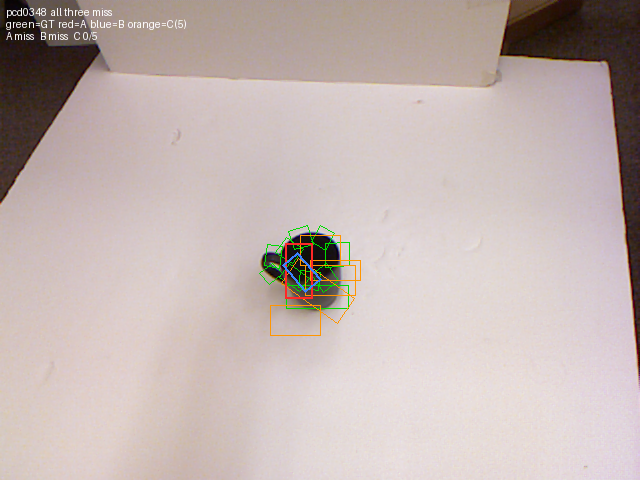
\includegraphics[width=0.8\textwidth]{compare_0348.png}
\caption{An orientation-only failure. The predicted grasping rectangle
correctly overlaps the object (intersection over union of 0.38) but
rotates 47 degrees from any labeled grasp. Of the four ResNet18
angle-only failures (pcd0676, pcd0348, pcd0824, pcd0316), only pcd0348
has a rendered sheet, which is why it was chosen.}
\label{fig:anglefail}
\end{figure}

The second round, in Table~\ref{tab:round2}, chose ResNet34 by a margin
of 0.2 validation points (81.4\% against 81.2\% mean final weights over
three seeds) and used augmentation, which lifted mean validation from
81.4\% to 83.3\%. On test the three ResNet34 seeds scored 84.6, 83.7,
and 83.7\%, a mean of 84.0\% with a standard deviation of 0.5. ResNet18
under the same recipe scored 83.7, 80.5, and 83.7\%, a mean of 82.6\%.
Re-running the first-round recipe at two new seeds gave
validation-selected checkpoints scoring 82.9\% and 80.5\% on test, so
the first round's 79.7\% was a low-side sample from a recipe whose seed
spread is about 1.6 points at the checkpoint and much larger at the
final weights, where the same two runs scored 80.5\% and 62.6\%.
Averaged final weights beat the validation-selected checkpoint of their
own run on five of six second-round runs. Test-time augmentation added
between 0.0 and 5.7 points across the six runs, about three on average.

\begin{table}[H]
\centering
\caption{System B, both rounds, on the same 123 test images. Round 2
numbers are means over three seeds of the final-epoch averaged weights;
no checkpoint was selected.}
\label{tab:round2}
\begin{tabular}{llr}
\toprule
Round & Configuration & Test accuracy \\
\midrule
1 & ResNet18, seed 42, best validation checkpoint & 79.7\% \\
1 & ResNet34, seed 42, best validation checkpoint & 70.7\% \\
1 recipe & ResNet18, seeds 0 and 1, best validation checkpoint & 82.9\%, 80.5\% \\
2 & ResNet18, three seeds, final weights, with augmentation & 82.6\% (83.7, 80.5, 83.7) \\
2 & ResNet34, three seeds, final weights, with augmentation & \textbf{84.0\%} (84.6, 83.7, 83.7) \\
\bottomrule
\end{tabular}
\end{table}

Object-clustered, round 2's 84.0\% has an interval of [73.9, 92.1]. It
leads System A by 26.3 points [14.8, 38.3], permutation $p = 0.0002$,
and System C by 71.7 points [61.3, 80.9]. Its 4.3-point lead over round
1 has an interval of [$-5.8$, $+13.7$] and does not exclude zero, so the
second round confirms the first-round result with measured uncertainty
and does not demonstrate an improvement. Round 1's nine-point advantage
of ResNet18 over ResNet34 is not supported, since the two architectures
perform equally within noise.

\subsection{System C}

System C achieved 12.4\% accuracy on test images (76 of 615 calls), with
a 95\% Wilson interval of [10.0, 15.2]. Each of the five independent
runs achieved 13.0\%, 14.6\%, 13.8\%, 10.6\%, and 9.8\% accuracy. The
best-of-five attempts achieved 35.0\% (43 of 123). A consensus rule that
scores whichever single repeat agrees most closely with the other four,
since continuous rectangles cannot be majority-voted directly, reached
12.2\%. Neither is the primary figure. Both require either multiple
calls per image or knowing the answer in advance. The model returned a
parseable reply on 614 of 615 calls (99.8\%), and every non-parsing call
counts as a miss in the primary figure.

\begin{table}[H]
\centering
\caption{Which criterion each prediction missed, computed through one
shared scoring path for all three systems.}
\label{tab:taxonomy}
\begin{tabular}{lrrr}
\toprule
Outcome & System A (of 123) & System B (of 123) & System C (of 615) \\
\midrule
Correct       & 71 (57.7\%) & 98 (79.7\%) & 76 (12.4\%) \\
Angle only    & 13 (10.6\%) &  4 (3.3\%)  & 85 (13.8\%) \\
Overlap only  & 18 (14.6\%) & 15 (12.2\%) & 88 (14.3\%) \\
Both          & 13 (10.6\%) &  6 (4.9\%)  & 365 (59.3\%) \\
No prediction &  8 (6.5\%)  &  0 (0.0\%)  & 1 (0.2\%) \\
\bottomrule
\end{tabular}
\end{table}

The failure taxonomy in Table~\ref{tab:taxonomy} shows where the three
systems differ most. For the geometric check described in Methods,
System C's predicted center fell outside the convex hull containing
every labeled grasp on 53.4\% of calls (328 of 614). System A showed
failures of this type on 7.0\% of the calls in which it attempted a
grasp (8 of 115 scored calls), and System B on 6.5\% (8 of 123).
Table~\ref{tab:hull} puts the three side by side.

\begin{table}[H]
\centering
\caption{Predicted grasp centers falling outside the convex hull of an
image's labeled grasps. This diagnostic is computed across all scored calls, so it overlaps the failure categories in Table~\ref{tab:taxonomy}.}
\label{tab:hull}
\begin{tabular}{lrr}
\toprule
System & Calls scored & Center outside hull \\
\midrule
System A &  115 &   8 (7.0\%)  \\
System B &  123 &   8 (6.5\%)  \\
System C &  614 & 328 (53.4\%) \\
\bottomrule
\end{tabular}
\end{table}

Agreement across System C's five runs was low. Mean self-agreement was
22.0\%, with a mean pairwise angle spread of 5.8 degrees and mean
pairwise intersection over union of 0.13. The distribution of how many
of five repeats scored correct per image appears in
Fig.~\ref{fig:repeats}. That puts 81 of 123 images (65.9\%) at a fully
consistent outcome, leaving 42 where the same model on the same pixels
sometimes passed and sometimes did not.

\begin{figure}[H]
\centering
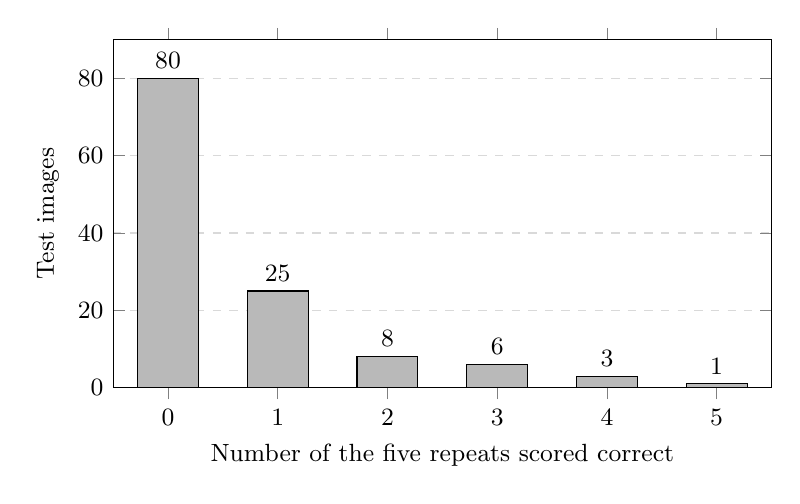
\begin{tikzpicture}
\begin{axis}[
  width=0.82\textwidth, height=6.0cm,
  ybar, bar width=22pt,
  ymin=0, ymax=90,
  xlabel={Number of the five repeats scored correct},
  ylabel={Test images},
  xtick={0,1,2,3,4,5},
  ymajorgrids=true, grid style={dashed,gray!30},
  nodes near coords, every node near coord/.append style={font=\small},
  tick label style={font=\small}, label style={font=\small},
]
\addplot[fill=gray!55,draw=black]
  coordinates {(0,80) (1,25) (2,8) (3,6) (4,3) (5,1)};
\end{axis}
\end{tikzpicture}
\caption{System C repeat consistency across 123 test images. On 80
images no repeat succeeded and on only one image did all five, leaving
42 images where the same model on the same pixels sometimes passed and
sometimes did not.}
\label{fig:repeats}
\end{figure}

Self-agreement provides some usable information. Restricting to the
21.1\% of images where at least 40\% of repeat pairs agreed lifts
best-of-five accuracy to 57.7\% on those images, against 35.0\% at full
coverage. The match with System A's single-prediction 57.7\% is
coincidental. This result indicates which of several repeated calls to
trust and is not comparable with the single-prediction accuracies of
Systems A and B.

\subsection{System D}\label{sec:res-d}

System D chose a passing candidate on 18.7\% of 615 calls (per repeat
17.1, 17.1, 17.9, 20.3, and 21.1\%), with a best-of-five of 39.0\%.
Every called reply parsed (560 of 560; the other 55 calls belong to the
eleven images with no candidates and count as misses).
Table~\ref{tab:som} sets that against the floor and ceiling of the same
menu, and Fig.~\ref{fig:som} shows one test image with the marks the
model saw. The paired object-clustered difference between System D and a
random choice from the same menu is $-1.4$ points [$-6.6$, $+4.0$].
System D's gain over System C's coordinate output, 6.3 points [$-1.6$,
$+15.0$], does not exclude zero either. The geometric rule in the fourth
row is statistically level with System A's post-hoc 57.7\% ($-2.4$
points [$-10.1$, $+5.4$]).

\begin{table}[H]
\centering
\caption{System D against the floor and ceiling of its own candidate
menu, and against System C, on the same 123 test images. Intervals are
object-clustered.}
\label{tab:som}
\begin{tabular}{lrr}
\toprule
 & Accuracy & 95\% CI \\
\midrule
System D, one call per image     & 18.7\% & [9.5, 29.7]  \\
Random choice among candidates   & 20.1\% & [14.6, 26.6] \\
Any candidate passes (ceiling)   & 79.7\% & [67.2, 90.0] \\
Geometric rule alone (candidate 0) & 55.3\% & [41.8, 68.0] \\
System C, one call per image     & 12.4\% & [8.0, 17.4]  \\
\bottomrule
\end{tabular}
\end{table}

\begin{figure}[H]
\centering
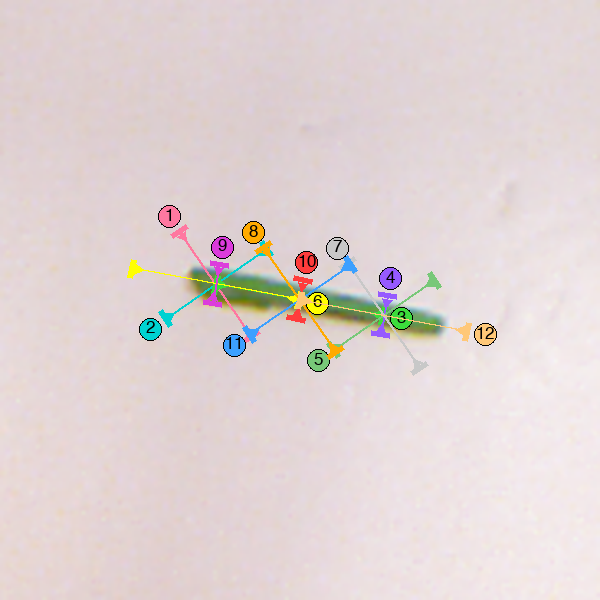
\includegraphics[width=0.62\textwidth]{som_0129.png}
\caption{The marked image for one test object as System D saw it. The
model chose mark 6, the yellow end pinch along the bean, on all five
repeats, describing it as gripping ``the central narrow part of the
bean''. Mark 10 crosses the bean at its centre and passes the metric.}
\label{fig:som}
\end{figure}

Self-agreement across the five repeats, measured on the physical
candidate with the numbering re-shuffled each call, was 44.3\%, twice
System C's. The preference it agreed on was for the candidate whose jaws
travel along the object's long axis near one end: 342 of 560 choices for
that single candidate, 391 for that orientation at any position. That
candidate type passes on 17.0\% of test images. The centroid candidate
closing across the short axis passes on 60.7\% and was chosen 34 times.
The model's stated confidence was ``high'' on 556 of 560 calls, of which
21\% were correct. The same preference had appeared during prompt
development on the 30 training images, in 34 of 58 calls with the first
glyph and 41 of 58 with the redesigned one.

The two follow-up menus are in Table~\ref{tab:menus}. On the
four-candidate menu drawn at real size the model scored 26.5\% against a
24.6\% random floor. With every mark the same size it scored 22.3\%
against the same floor. Neither paired difference excludes zero ($+1.9$
[$-2.2$, $+6.3$] and $-2.3$ [$-6.3$, $+1.7$]), nor does the difference
between the two menus ($+4.2$ [$-0.5$, $+9.4$]). The sparse menu's 7.8
point lead over the full menu excludes zero, but its floor is 4.5 points
higher, so the gain is attributable to the easier menu. On the
uniform-size menu the model chose the long-axis direction in 45\% of
calls against a 25\% chance rate, and the short-axis candidate, which
passes on 55\% of images, in 17\%.

\begin{table}[H]
\centering
\caption{System D on three candidate menus, same model, same 123 test
images, five repeats each. ``Long axis'' is the share of parsed calls
choosing the orientation whose jaws travel along the object's long
axis; chance is 25\% on the four-candidate menus.}
\label{tab:menus}
\begin{tabular}{lrrrrr}
\toprule
Menu & Marks & Accuracy & Random floor & Ceiling & Long axis chosen \\
\midrule
Full, three positions          & 12 & 18.7\% & 20.1\% & 79.7\% & 70\% \\
Centroid only, real size       &  4 & 26.5\% & 24.6\% & 65.9\% & 41\% \\
Centroid only, uniform size    &  4 & 22.3\% & 24.6\% & 65.9\% & 45\% \\
\bottomrule
\end{tabular}
\end{table}

\subsection{Cross-system comparison}

System A against System B is significant under McNemar's exact test (p =
1.4e-4), the 38-versus-11 split described below. System C was tested
separately against each of its five runs rather than pooled, and the
least significant of the five is reported, p = 5e-12 against System A
and p = 1.6e-20 against System B.

Every interval quoted so far treats images, or in System C's case
individual calls, as independent. They are not, because the 123 test
images sit inside 35 objects. Resampling whole objects with replacement
widens all of them. System A becomes [46.2, 68.2], System B [70.8,
87.1], System C [8.0, 17.4], and System C's best-of-five [24.6, 45.5].
Checking whether two such intervals overlap is a weak test, so the
differences were bootstrapped directly on the same resamples. System B
leads System A by 22.0 points [9.7, 35.1], System A leads System C's
best-of-five by 22.8 points [9.2, 35.6], and System A leads System C at
one call per image by 45.4 points [33.8, 55.6]. None of those intervals
contains zero, and an object-clustered permutation test agrees at p =
0.003, 0.006, and 5e-5. The ordering of the three systems survives the
change of sampling unit. The Wilson intervals reported per system above
are image-level and should be read as the narrower of the two.

Systems A and B agreed on 74 of 123 images, both correct on 60 and both
wrong on 14. Of the 49 they disagreed on, System B alone was correct on
38 and System A alone on 11. Counting System C as correct whenever any
of its five repeats passed, all three systems succeeded together on 22
images and failed together on 10. Fig.~\ref{fig:threeway} shows one such
image with all three systems overlaid.

\begin{figure}[H]
\centering
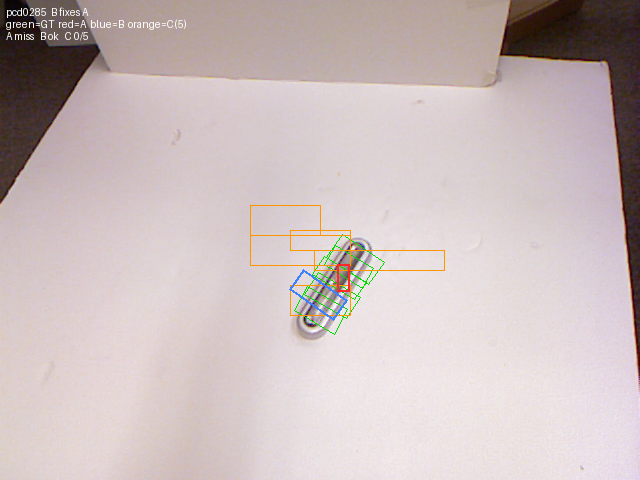
\includegraphics[width=0.8\textwidth]{compare_0285.png}
\caption{All three systems on one image. Labeled ground-truth grasps
are green, System A red, System B blue, and System C's five repeats
orange.}
\label{fig:threeway}
\end{figure}

\subsection{Orientation and label-count strata}\label{sec:res-strata}

Fig.~\ref{fig:strata} splits the test set by orientation. Relative to
the 103 axis-aligned images, System A dropped 21.2 points on the 20
diagonal images, System B gained 12.3 points, and System C moved 2.0
points. System A does not fall to zero on the diagonal stratum because
the 15 degree stratum rule is tighter than the 30 degree scoring
tolerance, so some diagonal images remain reachable by an axis-aligned
rectangle.

\begin{figure}[H]
\centering
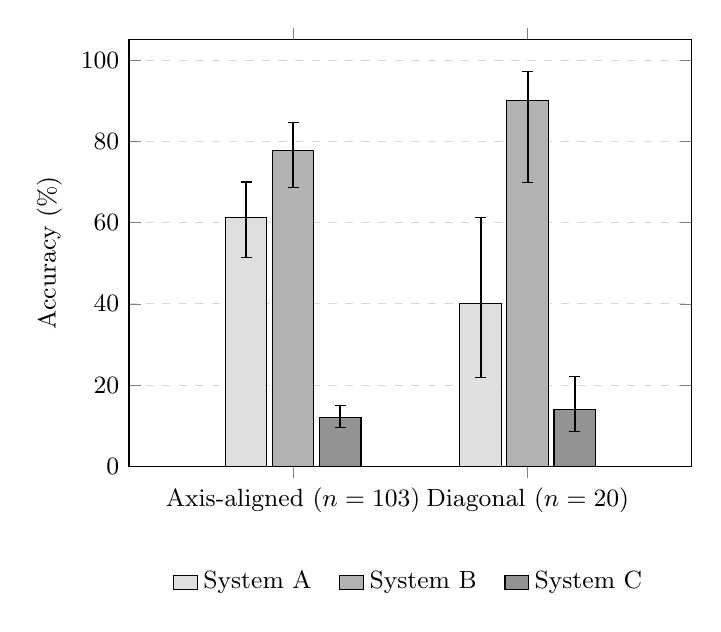
\begin{tikzpicture}
\begin{axis}[
  width=0.72\textwidth, height=7.0cm,
  ybar, bar width=15pt,
  ymin=0, ymax=105,
  symbolic x coords={axisaligned,diagonal},
  xtick=data,
  xticklabels={Axis-aligned ($n=103$), Diagonal ($n=20$)},
  enlarge x limits=0.7,
  ylabel={Accuracy (\%)},
  ymajorgrids=true, grid style={dashed,gray!30},
  legend style={at={(0.5,-0.22)}, anchor=north, legend columns=3,
                draw=none, font=\small, /tikz/every even column/.append style={column sep=8pt}},
  legend image code/.code={\draw[#1,draw=black]
     (0cm,-0.09cm) rectangle (0.30cm,0.09cm);},
  tick label style={font=\small}, label style={font=\small},
  error bars/error bar style={black,thick},
]
\addplot[fill=gray!25,draw=black,
  error bars/.cd, y dir=both, y explicit]
  coordinates {
    (axisaligned, 61.2) += (0,8.8)  -= (0,9.7)
    (diagonal,    40.0) += (0,21.3) -= (0,18.1)
  };
\addplot[fill=gray!60,draw=black,
  error bars/.cd, y dir=both, y explicit]
  coordinates {
    (axisaligned, 77.7) += (0,6.9)  -= (0,9.0)
    (diagonal,    90.0) += (0,7.2)  -= (0,20.1)
  };
\addplot[fill=gray!85,draw=black,
  error bars/.cd, y dir=both, y explicit]
  coordinates {
    (axisaligned, 12.0) += (0,3.1)  -= (0,2.5)
    (diagonal,    14.0) += (0,8.1)  -= (0,5.5)
  };
\legend{System A, System B, System C}
\end{axis}
\end{tikzpicture}
\caption{Accuracy by orientation stratum with 95\% Wilson intervals.
Axis-aligned, 103 images: System A 61.2 [51.5, 70.0], System B 77.7
[68.7, 84.6], System C 12.0 [9.5, 15.1]. Diagonal, 20 images: System A
40.0 [21.9, 61.3], System B 90.0 [69.9, 97.2], System C 14.0
[8.5, 22.1]. These are image-level rather than object-clustered, so
they are the narrower reading. The three systems move in three
directions, but the diagonal intervals are already wide enough that
only System A's drop, which was predicted from its representation
beforehand, should carry weight.}
\label{fig:strata}
\end{figure}

All three systems performed worst on the images with the most labeled
grasps (8 to 25), not the fewest, which is the opposite of what a
more-labels-means-easier-match hypothesis would predict. In that group,
System A scored 48.0\%, System B 64.0\%, and System C 11.2\%.

% ===============================================================
\section{Discussion}\label{sec:discussion}

\subsection{From the coordinate-binding hypothesis to System D}

The most distinctive feature of System C's errors is their location.
Most of its calls failed the angle and the overlap criterion together
(Table~\ref{tab:taxonomy}), and its predicted center fell outside the
convex hull of the labeled grasps far more often than either other
system's (Table~\ref{tab:hull}). The comparison is not fully even, since
System B was trained on this distribution and System A's center comes
from a detected box or a segmentation, so both almost always place the
center on the object, whereas System C is free to place a center
anywhere in the image. In a sample of failures, the model's written
explanation frequently named a real part of the object while the
coordinates in the same reply fell elsewhere in the image. That reading
was informal and not a blinded coding study with a fixed rubric, so it
is reported only as the observation that motivated a hypothesis, and the
frequency of the pattern was not measured. Wang et al.~\cite{wang2025}
document the same disconnect in an unrelated domain, with models
describing a correct solution to a visual puzzle in text, then clicking
hundreds of pixels away from it (their section 5.3.2). Together these
suggested that GPT-4o could see where to grasp but could not bind that
choice to pixel coordinates.

This explanation predicts that removing System C's coordinate output
should help if the problem is binding reasoning to coordinates, and
should make no difference if the problem is perception of the object.
System D ran that test, and the prediction was not borne out. Given a
menu of twelve candidates, GPT-4o chose a passing grasp no more often
than a uniformly random choice from the same menu, and its gain over its
own coordinate output does not exclude zero (Table~\ref{tab:som}). Two
published results had seemed consistent with the binding reading, though
neither was designed as a test of it. They remain relevant because they
show what a menu-based design can do when the menu and the model are
matched. Set-of-Mark lets zero-shot GPT-4V beat a fine-tuned specialist
on RefCOCOg purely by replacing coordinate output with region
selection~\cite{yang2024}. VLAD-Grasp scores far above System C on this
same dataset, training-free, by having the model draw the grasp instead
of stating it~\cite{kulshrestha2025}.

VLAD-Grasp is the published result most relevant to System C, but two
differences prevent a direct comparison with 12.4\%. First, it does not
only replace a coordinate with a picture. It then predicts depth,
segments the object, and aligns 3D point clouds to recover a pose, a
pipeline System C has no equivalent to. Second, it counts a grasp
correct on overlap alone, with no angle requirement, and reports 91.4\%
under that looser test on a set of 70 unseen Cornell objects. That the
same evaluation scores GR-ConvNet at 72.1\%, against the 97.7\%
GR-ConvNet reports for itself, shows the two protocols are not directly
comparable. The dropped angle criterion is what matters here, since
orientation is the variable this paper's results depend on most. The
model also differs, since the current revision of that paper names GPT-5
as its primary model, so its result describes vision-language models
without coordinate output in general and cannot be attributed to GPT-4o.

Even with that caveat, the contrast between VLAD-Grasp and System D is
informative in a way System C alone was not. Both remove the coordinate
output, but only VLAD-Grasp succeeds, and it also adds depth,
segmentation, and geometric pose recovery, so the geometry contributes a
substantial share of that pipeline's performance. On the full menu, System D most often chose the candidate whose jaws travel along the
object's long axis near one end, a type of grasp that rarely passes the
metric, and seldom chose the centroid candidate closing across the short
axis, which passes most often (Section~\ref{sec:res-d}). Its reasoning
for the preferred choice was typically that it ``grips the narrow top
edge near the center of mass''. From a top-down photograph, two pads
straddling the end of an elongated object appear to pinch a narrow part.
In three dimensions the second finger would land on top of the object.
The model reported high confidence on nearly every call, whether or not
the choice was correct. The failure that the center-hull diagnostic
exposed in System C is therefore not explained by the coordinate output
alone, and it is more consistent with a failure of grasp reasoning from
a single 2-D view. One rendering explanation, mark size, was tested and
ruled out. With four candidates at the centroid and every mark drawn at
the same size, the model still chose the long-axis direction well above
the chance rate and the short-axis candidate below it
(Table~\ref{tab:menus}). The preference is weaker without end-straddling
candidates, so part of the full-menu result was the end-pinch illusion
specifically and part is a general preference for closing along the long
axis.

These controls do not establish that the model reads the marks as
intended. The glyph redesign and the uniform-size menu address two
specific rendering confounds, but the model could still misjudge the
direction in which a drawn candidate closes, and its description of an
end pinch as a grip on a narrow part is compatible with that. A direct
control would ask the model a purely perceptual question about the same
marks, for example which candidate closes across the object's short
axis. That question has a known answer from the candidate generator and
needs no grasp label. High accuracy on that question would indicate that
the failure lies in the grasp choice, whereas low accuracy would
implicate mark interpretation. The control has not been run, so the
claim made here is limited to the statement that removing the coordinate
output is not sufficient to recover performance. The single-view setting
may also matter. Zhou et al.\ study vision-language models that must
combine several agents' egocentric views into one spatial understanding,
and improve that ability with supervised and reinforcement
fine-tuning~\cite{zhou2026}. Whether a second viewpoint, or depth, would
change the grasp that GPT-4o chooses was not tested here.

\subsection{Comparison with published regression results}

System B's accuracy can appear low next to two published Cornell
results, but neither is an even comparison. GR-ConvNet reports 97.7\% image-wise
and 96.6\% object-wise on an extended 1,035-image version of Cornell
\cite{kumra2020}, and only the object-wise figure is on the same
footing as anything here. Redmon and Angelova report 84.9\%
object-wise~\cite{redmon2015}. GR-ConvNet is a pixel-wise method that predicts a grasp at every pixel in a single pass, whereas System B pools a backbone's features and regresses one rectangle for the whole
image, the same design Redmon and Angelova published, whose 84.9\%
object-wise score is the fairer target, as laid out in
Table~\ref{tab:redmon}. The remaining differences favor the published system, since Redmon and Angelova used RGB-D and roughly 3,000 augmented examples per
image, while System B used RGB only and 620 real training images.

\begin{table}[H]
\centering
\caption{System B compared with Redmon and Angelova's Direct
Regression, the closest published architecture.}
\label{tab:redmon}
\begin{tabular}{lll}
\toprule
 & Redmon and Angelova (2015) & System B \\
\midrule
Architecture         & Global regression & Global regression \\
Orientation encoding & sin/cos of twice the angle
                     & sin/cos of twice the angle \\
Input                & RGB-D & RGB only \\
Training data        & \textasciitilde{}3,000 augmented per image
                     & 620 real images \\
Backbone             & AlexNet & ResNet18, then ResNet34 \\
Object-wise accuracy & 84.9\% & 79.7\% (round 1), 84.0\% (round 2) \\
\bottomrule
\end{tabular}
\end{table}

\subsection{Orientation and label count}

The orientation split produced the pattern each design predicts
(Section~\ref{sec:res-strata}). Both effects are expected, since an
axis-aligned box cannot represent a diagonal grasp and the sine and
cosine encoding was designed to handle rotation. The value of the split
is as a diagnostic, a use for which no precedent was found. It checks
whether each system's accuracy rises or falls along an axis defined by
the dataset's own grasp-angle annotations, instead of reporting a single
train and test generalization number.

The diagonal stratum holds only 20 images, and the 95\% intervals around
System B's and System C's per-stratum accuracies are wide enough that
their point changes there are not reliably distinguishable from noise.
Only System A's drop was predicted from its representation before the
stratum was scored. Predicting a direction in advance is not the same as
confirming an effect, and no interaction test between system and stratum
was run, so this analysis remains exploratory. System C's near-flat
response is what a system with no working orientation signal would
produce.

The label-count split did not behave as a difficulty proxy. All three
systems performed worst on the images with the most labeled grasps. The
likely explanation is that annotators labeled more grasps on objects
that afford more of them, so the count reflects object complexity more
than the leniency of the metric.

\subsection{What the comparison adds}

None of the individual observations is new. The sine and cosine encoding
dates to 2015, learned models have outperformed rule-based baselines on
Cornell for a decade, and imprecise vision-language coordinates have
been documented elsewhere. The contribution of this experiment is to
quantify the last weakness on a standard benchmark against two
baselines, and then to test the most natural account of it and find it
insufficient. A side result of the menu is a rule that closes across the
segmented object's short axis at its centroid, with no learning and no
detector. It is statistically level with System A's post-hoc figure
(Table~\ref{tab:som}), and it is the only label-free baseline in this
study that can express a diagonal grasp.

The second training round also corrected an earlier interpretation. The
first round's nine-point gap between ResNet18 and ResNet34 had been
attributed to the smaller network suiting a small dataset. Three seeds
per architecture under a stable recipe placed them within 1.4 points of
each other. A single training run on 620 images, with a checkpoint
chosen from a hundred noisy validation epochs, does not provide evidence
about architecture.

A one-million-parameter network trained from scratch did not learn the
task adequately, reaching 23.6\% after a learning-rate sweep confirmed
that this was not a tuning artifact. It still exceeded GPT-4o (System C)
by 11 points, which was not anticipated.

Three defects in the evaluation code were caught before any result was
reported, each of which would have produced a plausible but wrong
number. Each was found when an automated result did not match an
independent calculation, and neither value was used until the
disagreement was explained.

% ===============================================================
\section{Limitations}

This study used a single split of the dataset, whereas most published
Cornell results use five-fold cross-validation. Seven of the 35 object
groups in the test split contain only a single image of the object, so
the results for those objects are imprecise. The test split was opened
twice for System B, once per round, and the second round's selection
rules were fixed beforehand so that the second opening could not steer
any choice. The round-1 numbers rest on one seed each and the round-2
numbers on three. Jacquard, considered as a second dataset, was not
available during this study, so generalization across datasets was not
tested. An early formatting check on roughly 550 grasp rectangles likely
included a small number of images that were later assigned to the test
split. No threshold, constant, or lookup entry was derived from that
check.

The three systems did not receive comparable engineering effort, which
weakens any reading of this as a fully controlled comparison. System B
received three architectures, a five-point learning-rate sweep, a tuned
loss weight, and validation-based model selection. System C received one
prompt, frozen after development on 30 training images and never
revised. Freezing it protected test-set integrity, but prompt design is
the vision-language equivalent of architecture search, and architecture
search was run for one system and not the other. The 12.4\% figure
therefore measures what a single, un-iterated prompt achieves and should
not be read as a ceiling for zero-shot GPT-4o, although the gap to
System B is wide enough that prompt iteration is unlikely to reverse the
ordering. System D shares this limit and has a further one, since all
three menus came from one candidate generator and were drawn in one
glyph style on a zoomed crop. A different mark style, or marks placed by
a segmentation the model itself produced, was not tested. No control
measured whether the model reads the closing direction of a mark
correctly, so mark interpretation remains a possible contributor to
System D's result.

Cornell is public and widely mirrored, so GPT-4o may have been exposed
to it during training. When asked to name the source of ten test images
from different object categories, the model recognized none of them.
That is weak evidence against contamination. Contamination could only
have raised System C's score, which is already the lowest of the three,
so its ranking holds even in the worst case.

Every image-level and call-level interval and significance test reported
here treats its unit of analysis as independent, which does not hold
here. System C's interval is computed over 615 calls, but those calls
are five repeats of 123 images, so the interval is narrower than the
data support. The image-level intervals and McNemar tests for Systems A
and B have the same problem one level up, since the 123 test images are
grouped within 35 objects and images of one object are not independent
of each other. The stated population is unseen objects, so the correct
sampling unit is the object. The object-clustered intervals and
differences reported in the results section are the primary ones, and
the per-system Wilson intervals are image-level and should be read as
lower bounds on the uncertainty. Weighting each object equally rather
than by how many images it contributes lowers every system, System A to
51.3\%, System B to 75.4\%, and System C to 10.5\%, because test object
groups range from one image to nine, but the ordering of the systems
does not change.

The orientation analysis rests on only 20 diagonal images. The
vision-language results come from one model and one way of posing the
question, so they describe that setup and should not be extended to
vision-language models in general.

All systems received RGB images only, and no depth information was used.

% ===============================================================
\section{Conclusion}

A grasp decision can be written as rules, learned from labeled data, or
requested from a general-purpose vision-language model. These options
differ greatly in what they cost to build, and they are seldom measured
side by side. This paper built one system of each kind and scored all of
them with one implementation of the Cornell rectangle metric, on the
same 123 held-out images of 35 objects that none of them had seen, with
uncertainty computed at the level of the object.

The ordering was consistent across every analysis. A fine-tuned ResNet34
reached 84.0\% averaged over three seeds (a single-seed ResNet18 reached
79.7\% in the first round), a detector with a lookup table reached a
post-hoc-corrected 57.7\%, and zero-shot GPT-4o reached 12.4\%. The
manner in which each system failed is more informative than the accuracy
figures. The rule-based system usually finds the object but can only
place an axis-aligned rectangle, so it loses accuracy where the labeled
grasps run diagonally. The learned system orients well, to within about
eight degrees on its correct predictions, and most of its remaining
error is placement. GPT-4o fails at an earlier stage than either. More
than half of its predicted centers fall outside the region spanned by
all labeled grasps, often while its own text describes a sensible part
of the object.

That pattern suggested a model that sees the right grasp and cannot
express it in pixels. The marked-candidate experiment tested that
account and did not support it. Given numbered candidates to choose
from, with a ceiling of 79.7\%, the same model performed at the random
floor of the menu on three menus, and it consistently preferred a pinch
along the object's long axis, which resembles a grip on a narrow part
only when viewed from above. Removing the coordinate output is therefore
not sufficient to recover performance. The evidence points to the grasp
choice itself, although the model's reading of the drawn marks has not
been measured separately.

These results have three practical implications. First, a hosted
vision-language model prompted once for a grasp pose is not yet a
substitute for even a simple heuristic, which is consistent with
published systems that use such models to choose an object or a part and
leave the pose to geometry. Second, a label-free rule that closes across
the short axis of the segmented object matched the detector-based
baseline and can express diagonal grasps, which makes it a stronger
low-cost baseline than a lookup table. Third, results on a benchmark of
this size are sensitive to the training seed and to the unit of
analysis. A nine-point gap between two architectures disappeared under
three seeds, and every interval widened once images were clustered by
object, so multiple seeds and object-level clustering are recommended
for work at this scale. The next steps are a perceptual control on the
candidate marks, depth or multi-view input, newer models, and a second
dataset.

% ===============================================================

\newpage
\begin{thebibliography}{99}\addcontentsline{toc}{section}{Bibliography}
\bibitem{jiang2011} Y. Jiang, S. Moseson, and A. Saxena, ``Efficient grasping from RGBD images: Learning using a new rectangle representation,'' in \emph{Proc. IEEE ICRA}, 2011, pp. 3304--3311.
\bibitem{lenz2015} I. Lenz, H. Lee, and A. Saxena, ``Deep learning for detecting robotic grasps,'' \emph{Int. J. Robot. Res.}, vol. 34, nos. 4--5, pp. 705--724, 2015.
\bibitem{redmon2015} J. Redmon and A. Angelova, ``Real-time grasp detection using convolutional neural networks,'' in \emph{Proc. IEEE ICRA}, 2015, pp. 1316--1322.
\bibitem{morrison2018} D. Morrison, P. Corke, and J. Leitner, ``Closing the loop for robotic grasping: A real-time, generative grasp synthesis approach,'' in \emph{Robotics: Science and Systems XIV}, 2018.
\bibitem{kumra2020} S. Kumra, S. Joshi, and F. Sahin, ``Antipodal robotic grasping using generative residual convolutional neural network,'' in \emph{Proc. IEEE/RSJ IROS}, 2020, pp. 9626--9633.
\bibitem{he2016} K. He, X. Zhang, S. Ren, and J. Sun, ``Deep residual learning for image recognition,'' in \emph{Proc. IEEE CVPR}, 2016, pp. 770--778.
\bibitem{ren2015} S. Ren, K. He, R. Girshick, and J. Sun, ``Faster R-CNN: Towards real-time object detection with region proposal networks,'' in \emph{Adv. Neural Inf. Process. Syst.}, vol. 28, 2015.
\bibitem{openai2024} OpenAI, ``GPT-4o system card,'' arXiv:2410.21276, 2024.
\bibitem{yang2024} J. Yang et al., ``Set-of-Mark prompting unleashes extraordinary visual grounding in GPT-4V,'' arXiv:2310.11441, 2023.
\bibitem{kulshrestha2025} M. Kulshrestha et al., ``VLAD-Grasp: Zero-shot grasp detection via vision-language models,'' arXiv:2511.05791, 2025.
\bibitem{jiao2025} R. Jiao et al., ``Free-form language-based robotic reasoning and grasping,'' arXiv:2503.13082, 2025.
\bibitem{mirjalili2023} R. Mirjalili et al., ``Lan-grasp: Using large language models for semantic object grasping and placement,'' arXiv:2310.05239, 2023.
\bibitem{qian2024} Y. Qian et al., ``ThinkGrasp: A vision-language system for strategic part grasping in clutter,'' arXiv:2407.11298, 2024.
\bibitem{wang2025} J. Wang et al., ``COGNITION: From evaluation to defense against multimodal LLM CAPTCHA solvers,'' arXiv:2512.02318, 2025.
\bibitem{zhou2026} H. Zhou et al., ``Ego to World: Collaborative spatial reasoning in embodied systems via reinforcement learning,'' arXiv:2603.14811, 2026.
\end{thebibliography}

\section*{Acknowledgment}\addcontentsline{toc}{section}{Acknowledgment}

GPT-4o is the model studied as System C and System D. Separately,
Anthropic's Claude Code was used as a coding and writing assistant
throughout this project. It helped write and debug the code, made a
first pass at the ambiguous object boundaries, which I then audited by
hand as described in the Methods, implemented the second training round
and System D under my design, and helped draft and edit the text. OpenAI
Codex helped shorten a conference version. I chose the question,
designed the study, made the research decisions, ran and checked the
experiments, and verified the numbers and citations. A five-page version
of this work was submitted to the IEEE ICDM 2026 Teen Research
Symposium. I thank Heng Zhou and Manav Kulshrestha for comments on the
first version of this preprint, which led to the reorganization and the
narrower System D claim in this version.

\end{document}
